\documentclass[12pt,parskip=full]{article}
\usepackage{lmodern}
\usepackage{amsmath}
\usepackage[left=1.0in,right=1.0in,top=0.5in,bottom=1.0in]{geometry}
\geometry{letterpaper}
\usepackage{graphicx}
\usepackage{caption}
\usepackage{subcaption}
\usepackage{longtable}
\usepackage{float}
\usepackage{wrapfig}
\usepackage{soul}
\usepackage{textcomp}
\usepackage{marvosym}
\usepackage{wasysym}
\usepackage{latexsym}
\usepackage{amssymb}
\usepackage{apacite}
\usepackage{tabu}
\usepackage[svgnames]{xcolor}
\usepackage{tikz}
\usepackage[linktoc=all]{hyperref}
\usepackage{cleveref}
\usepackage{listings}
\usepackage{setspace}
\usepackage{parskip}
\usepackage{array}
\usepackage{apacite}
\usepackage{natbib}
\usepackage{multicol}
\usepackage{subcaption}
\usepackage{mathtools}
\usetikzlibrary{arrows}

\pgfdeclarelayer{edgelayer}
\pgfdeclarelayer{nodelayer}
\pgfsetlayers{edgelayer,nodelayer,main}

\tikzstyle{none}=[inner sep=0pt]
\tikzstyle{waypt}=[circle,fill=Black,draw=Black,scale=0.4]
\tikzstyle{Helobody}=[circle,fill=White,draw=Black,scale=4.0]
\tikzstyle{Tailrotor}=[circle,fill=White,draw=Black,scale=1.0]
\tikzstyle{ForceVector}=[->,draw=Indigo,fill=Indigo]
\tikzstyle{Coordinate}=[->,draw=Red,fill=Red,fill opacity=1.0]
\tikzstyle{angle}=[->]
\tikzstyle{MeasureMark}=[|-|]
\newlength{\imagewidth}
\newlength{\imagescale}

\setlength{\parskip}{11pt}
%\setlength{\parindent}{15pt}
\usepackage{bookmark}
\makeatletter
%\renewcommand\@seccntformat[1]{}
\makeatother

\lstset
{
	language=c,
	keywords={break,case,catch,continue,else,for,
		if,return,switch,try,while,int,void},
	basicstyle=\ttfamily,
	keywordstyle=\color{blue},
	commentstyle=\color{ForestGreen},
	stringstyle=\color{purple},
	numbers=left,
	numberstyle=\tiny\color{gray},
	stepnumber=1,
	numbersep=10pt,
	backgroundcolor=\color{white},
	tabsize=4,
	showspaces=false,
	showstringspaces=false
}

\renewcommand{\thesection}{\arabic{section}}

\renewcommand{\thesubsection}{\thesection\alph{subsection}}
\renewcommand{\theequation}{\thesubsection\arabic{equation}}
\newcommand*\circled[1]{\tikz[baseline=(char.base)]{
			\node[shape=circle,draw,inner sep=1pt] (char) {#1};}}
			
\numberwithin{subsection}{section}

\begin{document}
	\vspace{-4ex}
	\title{EbbCFD Theory Guide Part 2\vspace{-3.5ex}}
	\author{Rob Rau\vspace{-4ex}}
	\date{\today\vspace{-4ex}}
	\maketitle

	\section{Introduction}
		The last three months of work on EbbCFD have focused on 3 primary goals: Improvements to the plotting system in order to
		better display higher order results, implement viscous flux terms in order to compute the full compressible Navier-Stokes 
		equations, and finally to empirically demonstrate the accuracy and convergence rate of EbbCFD.

	\section{High Order Plotting}
		Previously, EbbCFD could only plot cell averaged values, throwing away any additional information used used by the solver.
		The current solver also uses cell centered solution gradients and edge mid-point solution values. With this information
		a better solution estimate can be displayed.
		
		To address this ebb-reconstruct was developed in order to generate higher order visualizations. To do this, ebb-reconstruct
		breaks up each $N$ edge cell into $2N$ triangles. The vertices used for these new triangles are the cell centroid, the edge
		mid-points and the actual cell vertices. It then uses the cell centered gradients to interpolate solution values to the new
		vertices. Edge mid-points and cell vertices have multiple values associated with them after this step so the final value is
		the average of all values associated with a point.

		\begin{figure}[H]
			\centering
			\begin{subfigure}{0.4\textwidth}
				\hspace*{-2cm}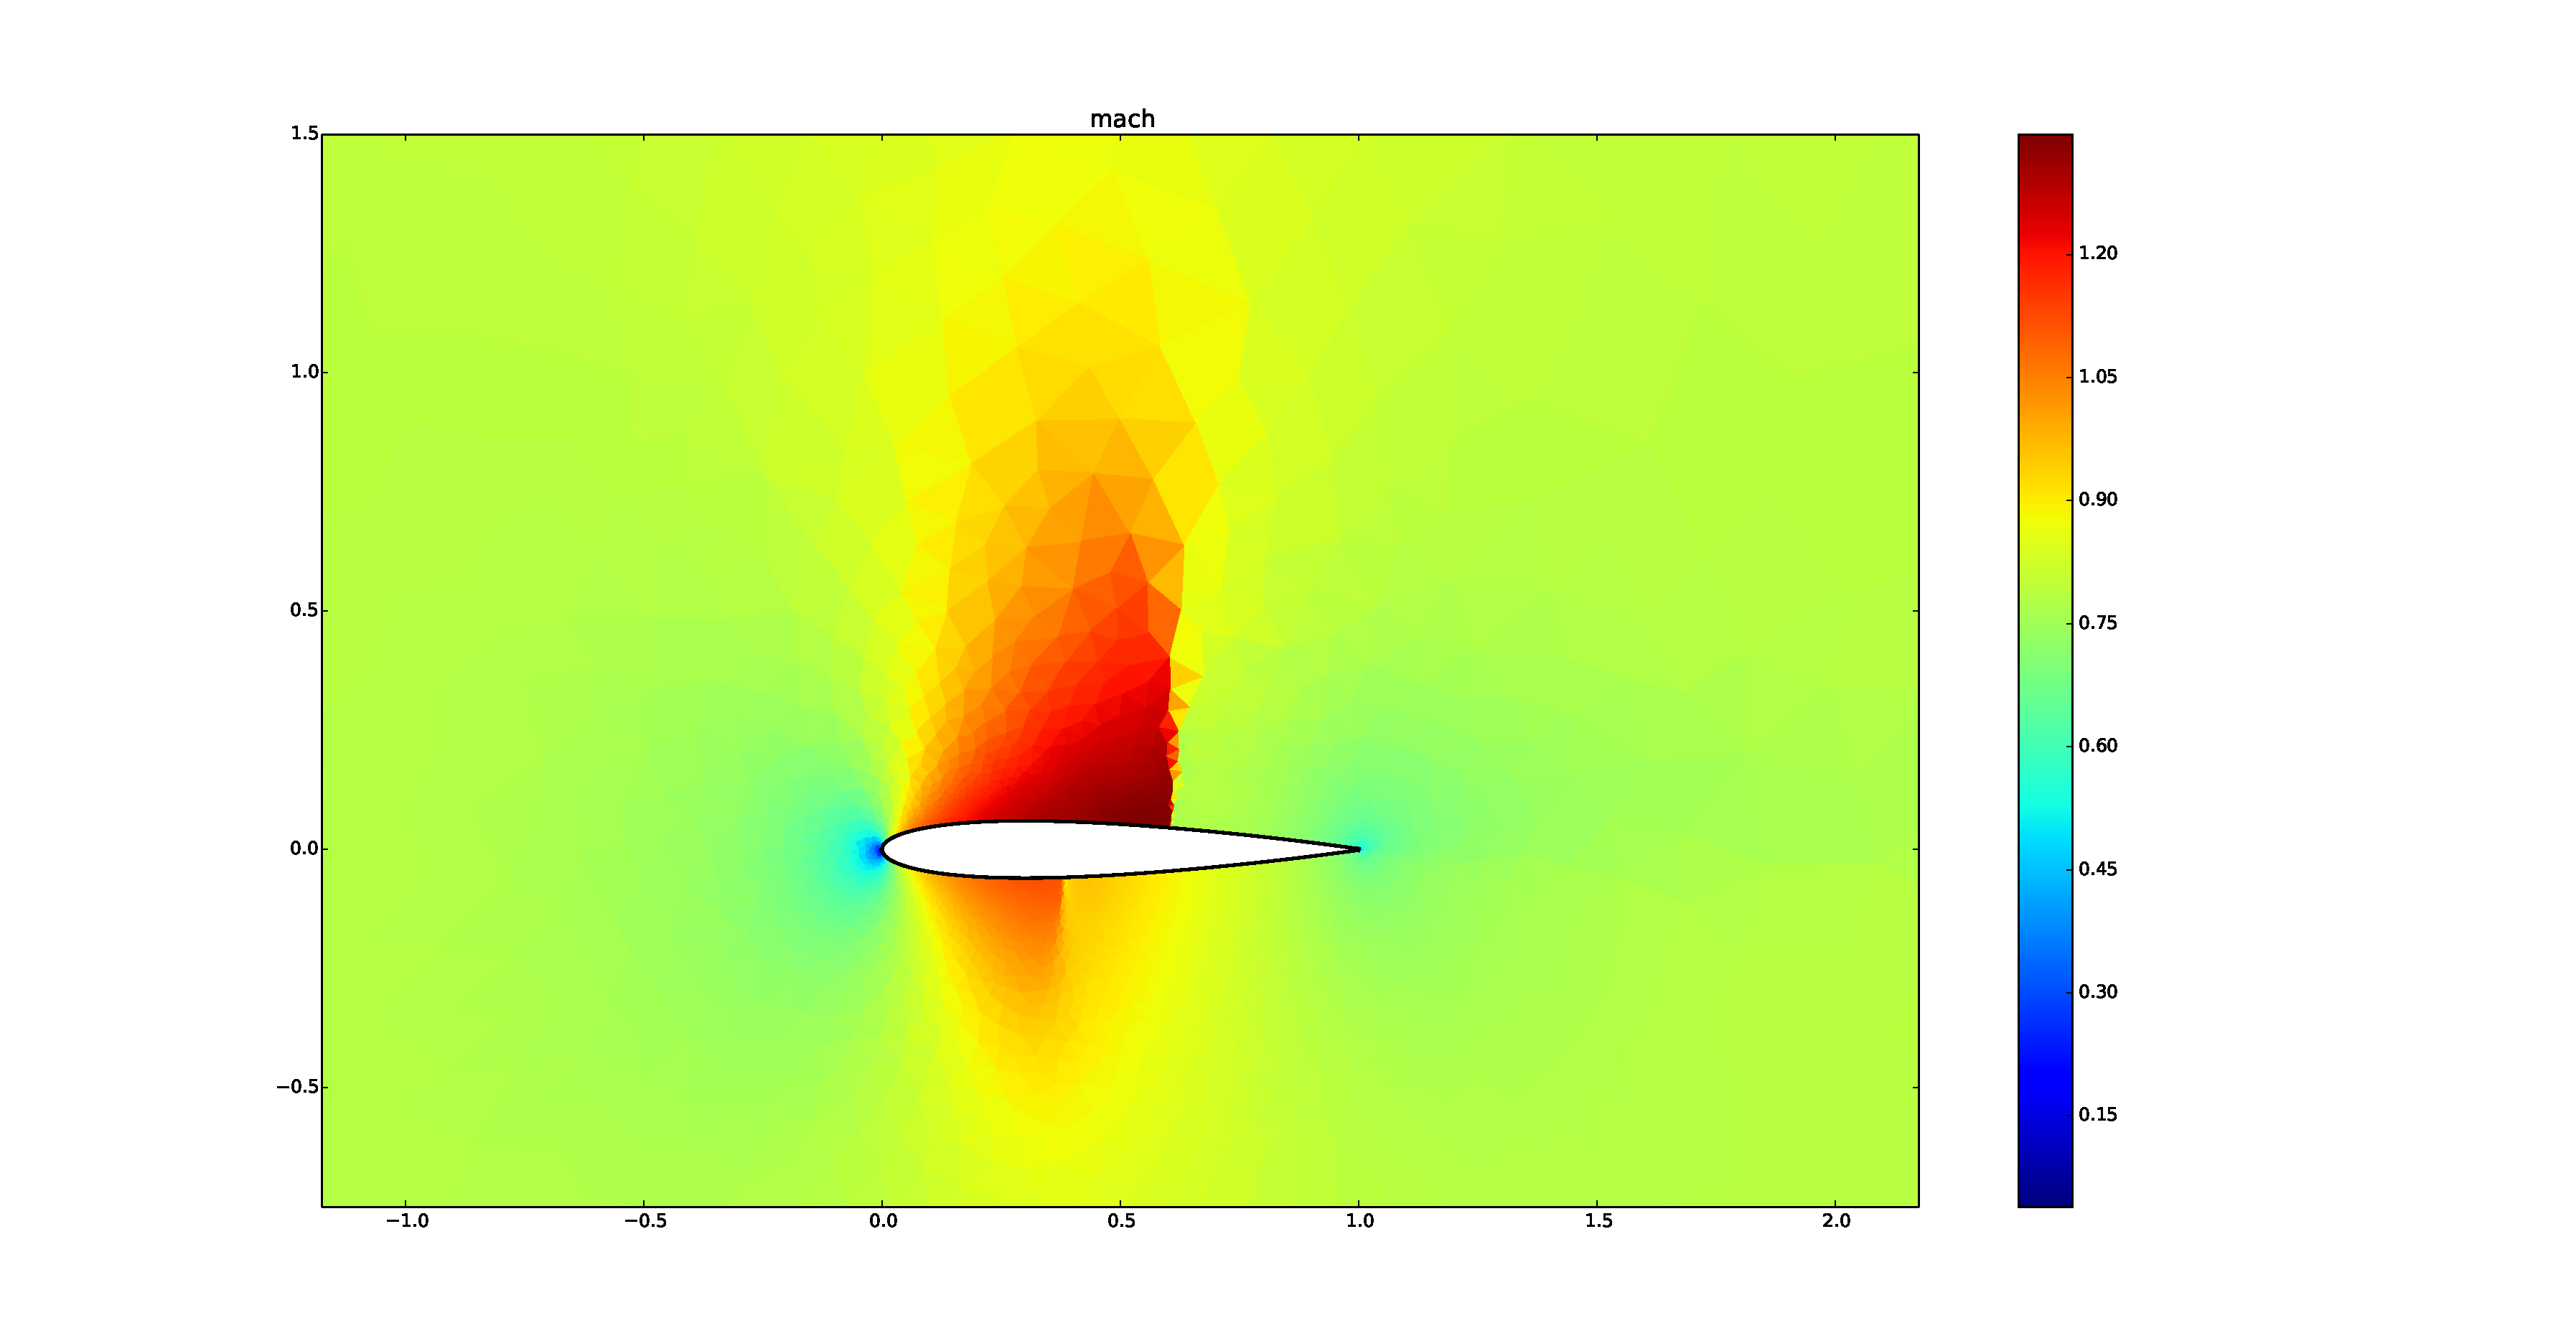
\includegraphics[scale=0.2,trim={7cm 2cm 10cm 2cm},clip]{CellAvgPlot.pdf}
				\hspace*{-2cm}\caption{Displaying only cell average values}
			\end{subfigure}
			\begin{subfigure}{0.4\textwidth}
				\hspace*{1cm}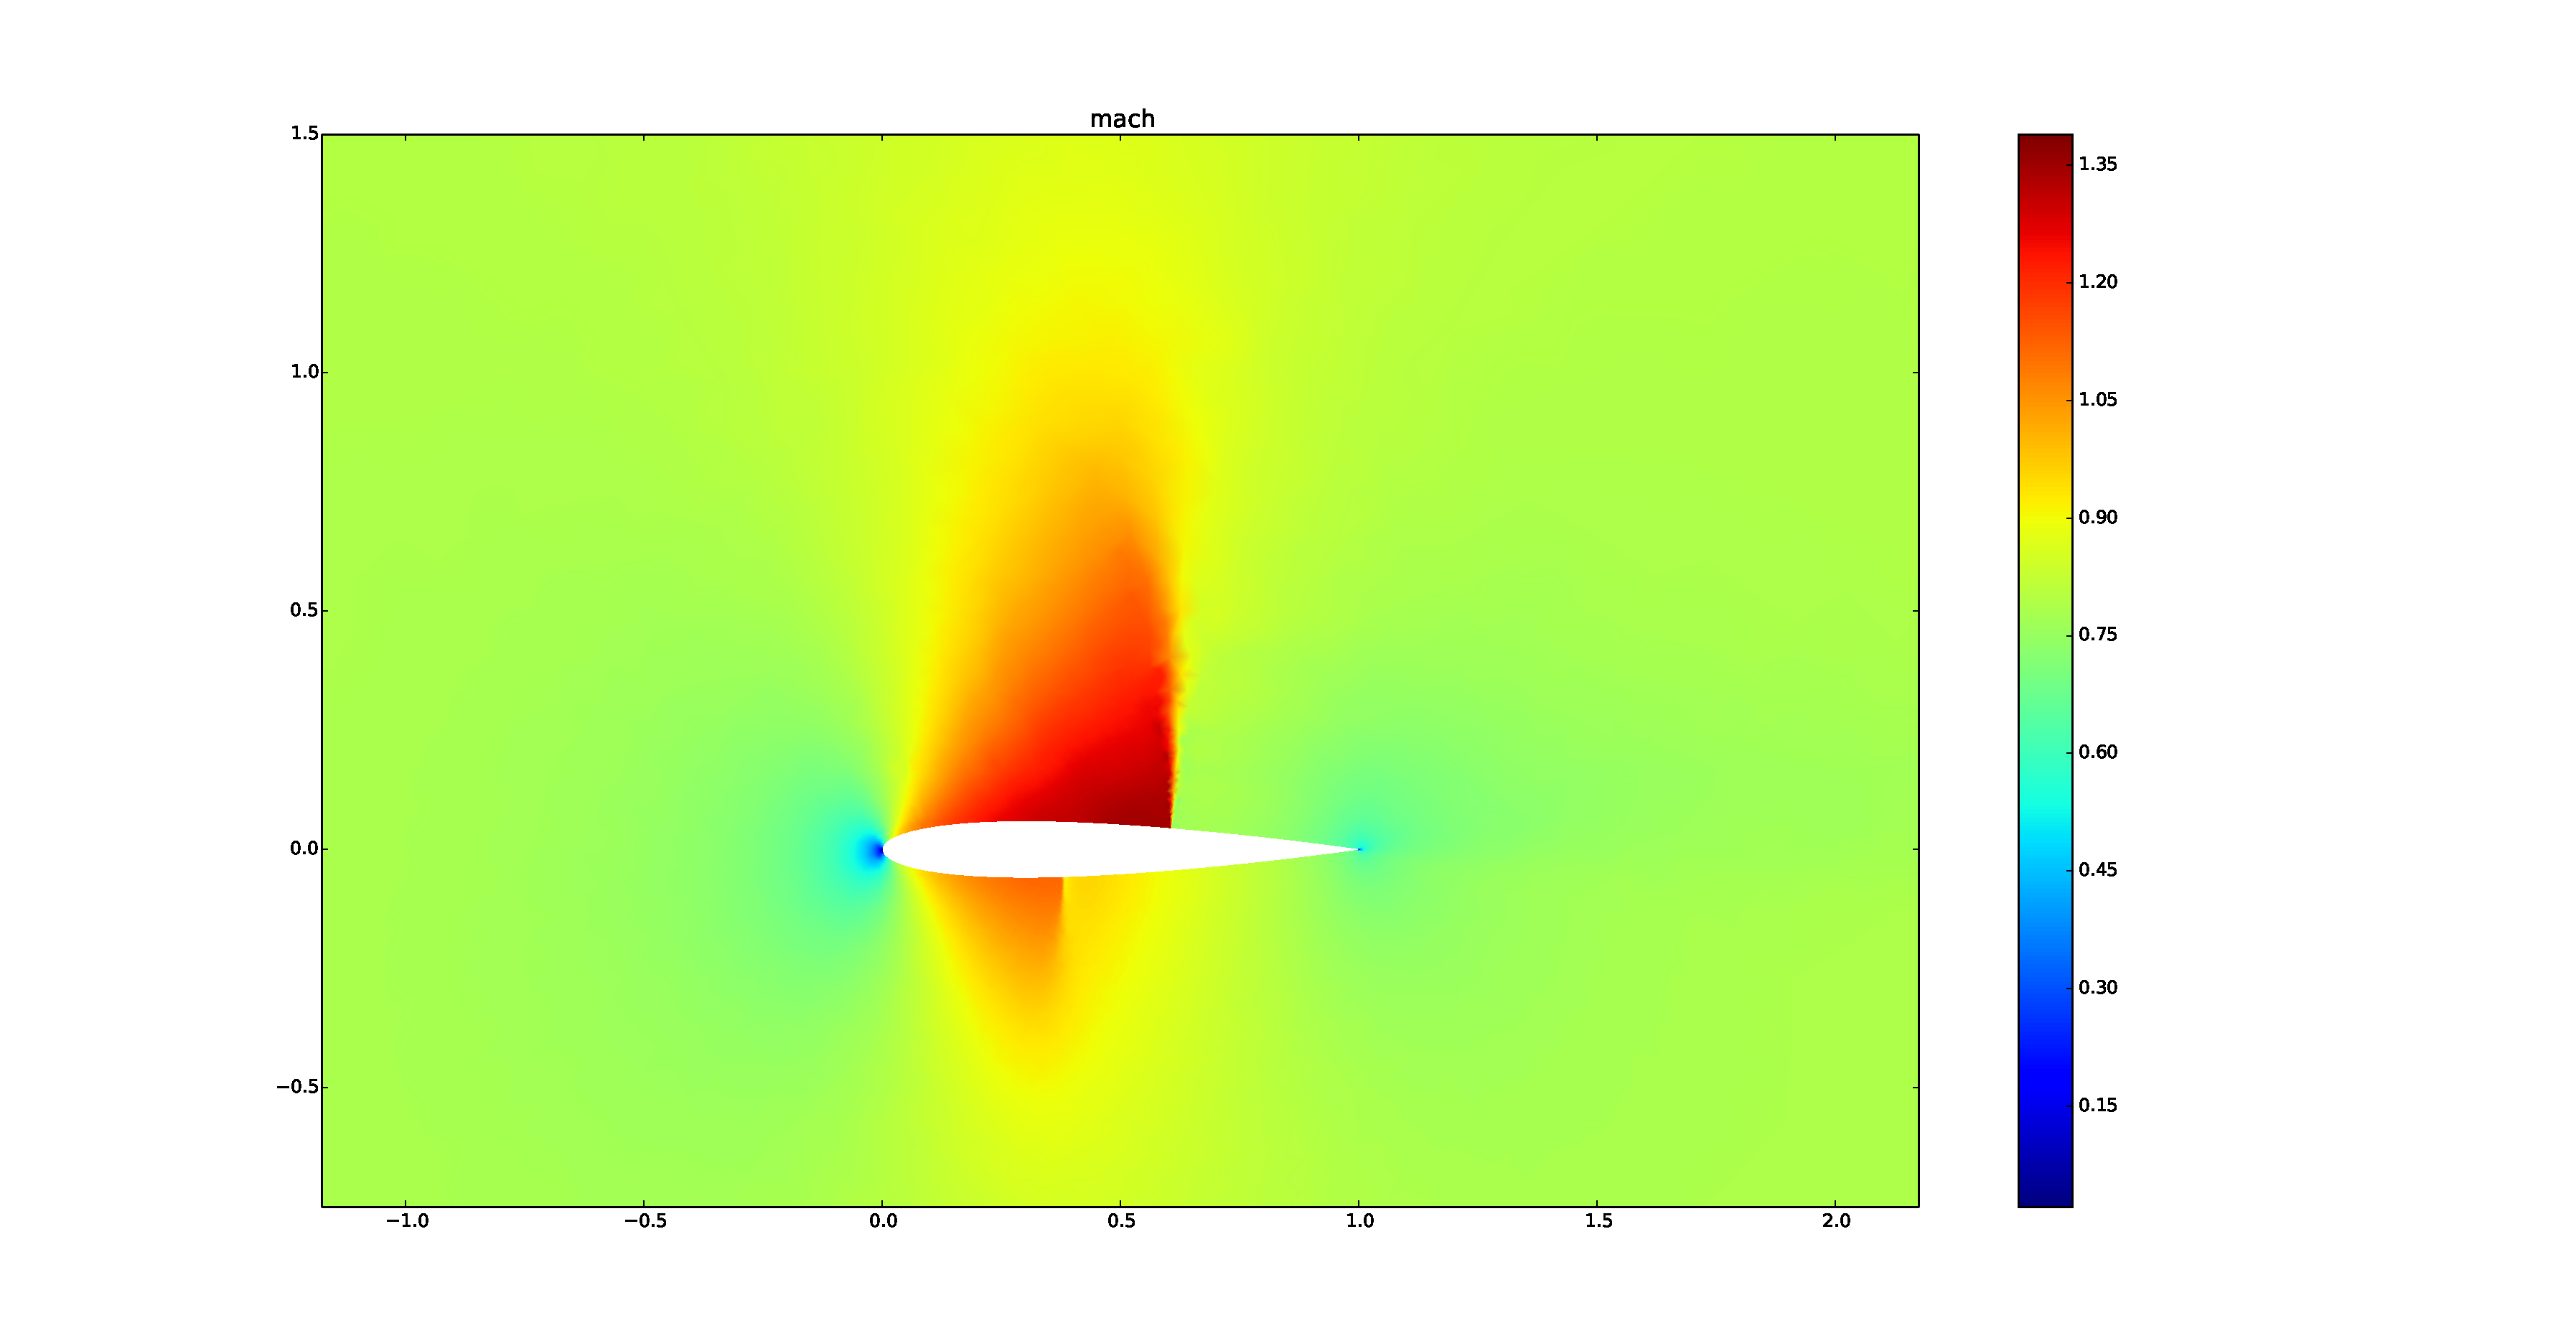
\includegraphics[scale=0.2,trim={7cm 2cm 10cm 2cm},clip]{ReconstructedPlot.pdf}
				\hspace*{1cm}\caption{Displaying reconstructed solution}
			\end{subfigure}
		\end{figure}
		
	\section{Navier-Stokes}
		To compute the diffusive flux terms needed by the Navier-Stokes equations, EbbCFD takes a very simple approach that only uses
		values already computed by the second order solver. To compute the diffusive flux at the cell edges, the solution gradients
		are also required at the cell edges. To do this, EbbCFD takes the cell centered solution gradients computed for second order
		and averages them with the neighboring cells solution gradients. This resulting average is then used to compute the diffusive
		flux matrices. For boundary edges, mainly walls, the cell centered gradient is directly used. As shown later, this produces 
		a second order accurate Navier-Stokes solver on regular-quadrilateral grids. Convergence on irregular grids has not been tested yet.
		
		To show that the Navier-Stokes solution is accurate a flat plate simulation was performed and the drag results were compared to the
		Blassius solution.

		\begin{figure}[H]
			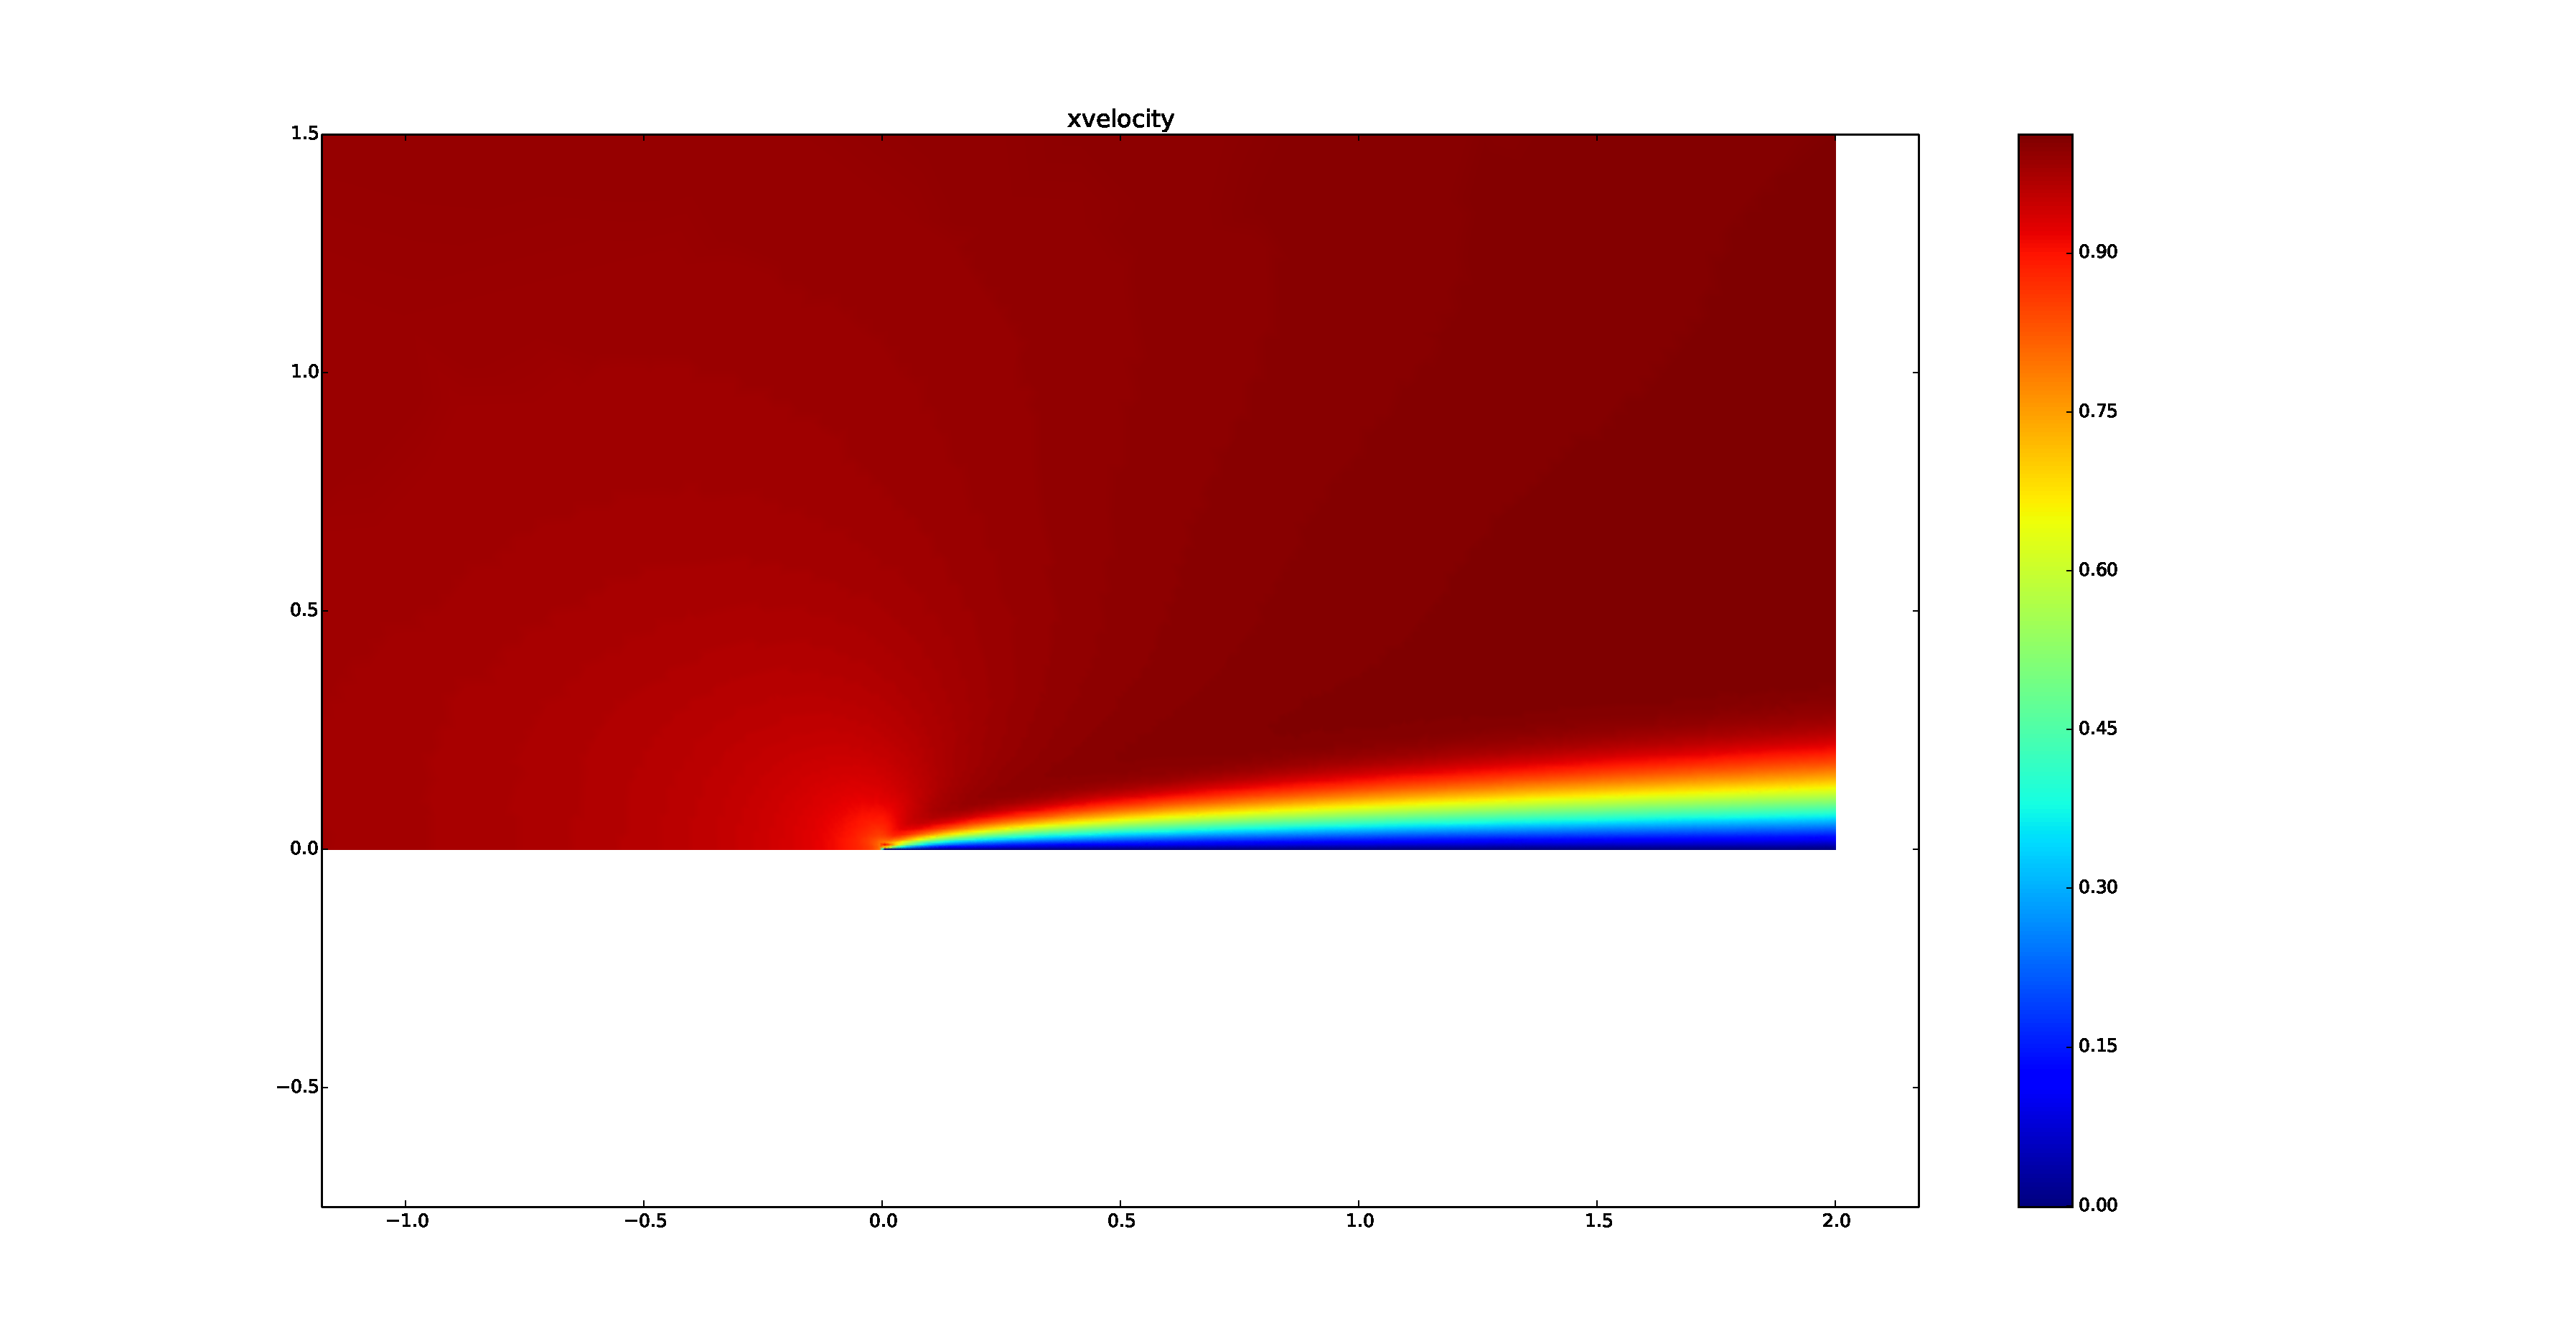
\includegraphics[width=\textwidth]{FlatPlate.pdf}
		\end{figure}
		
		The computed drag coefficient of this solution is within $\%5.6$ of the actual Blassius solution.

	\section{Method of Manufactured Solutions}
		To show that EbbCFD had correctly implemented its discritization, I employed the Method of Manufactured Solutions. This method allows
		one to prescribe an exact solution to the equations being solved. For steady state Navier-Stokes, we are solving the following equations
		\begin{equation}
			0 = \nabla \cdot \boldsymbol{F}(\boldsymbol{u}) - \nabla \cdot \boldsymbol{G}(\boldsymbol{u}, \partial\boldsymbol{u})
		\end{equation}
		where $\boldsymbol{F}(\boldsymbol{u})$ is the convective flux and $\boldsymbol{G}(\boldsymbol{u}, \partial\boldsymbol{u})$ is the viscous flux.
		When a solution is prescribed to this equation however one will find that it in-fact equals
		\begin{equation}
			\boldsymbol{S}^{MS} = \nabla \cdot \boldsymbol{F}(\boldsymbol{u}) - \nabla \cdot \boldsymbol{G}(\boldsymbol{u}, \partial\boldsymbol{u})
		\end{equation}

		If we subtract off the new source term from what EbbCFD solves itself, we can then get a good idea of the convergence characteristics.

		The exact solution chosen was
		\begin{align}
			\rho &= a_\rho + b_\rho \sin(c_\rho x + d_\rho y) \\
			u &= a_u + b_u \cos(c_u x + d_u y) \\
			v &= a_v + b_v \cos(c_v x + d_v y) \\
			p &= a_p + b_p \sin(c_p x + d_p y)
		\end{align}

		Convergence tests for the Euler equations were carried out on a variety of grids and configurations to thoroughly vet the code. The following
		configurations were used.
		
		\begin{itemize}
			\item Euler Uniform quadrilateral grid
			\item Euler Uniform triangular grid
			\item Euler Perturbed triangular grid
			\item Euler Uniform triangular grid with limiter
			\item Euler Uniform triangular grid with LP limiter
			\item Euler Uniform quadrilateral grid with limiter
			\item Euler Uniform quadrilateral grid with LP limiter
			\item Navier-Stokes Uniform quadrilateral grid
		\end{itemize}
		
		\begin{figure}[H]
			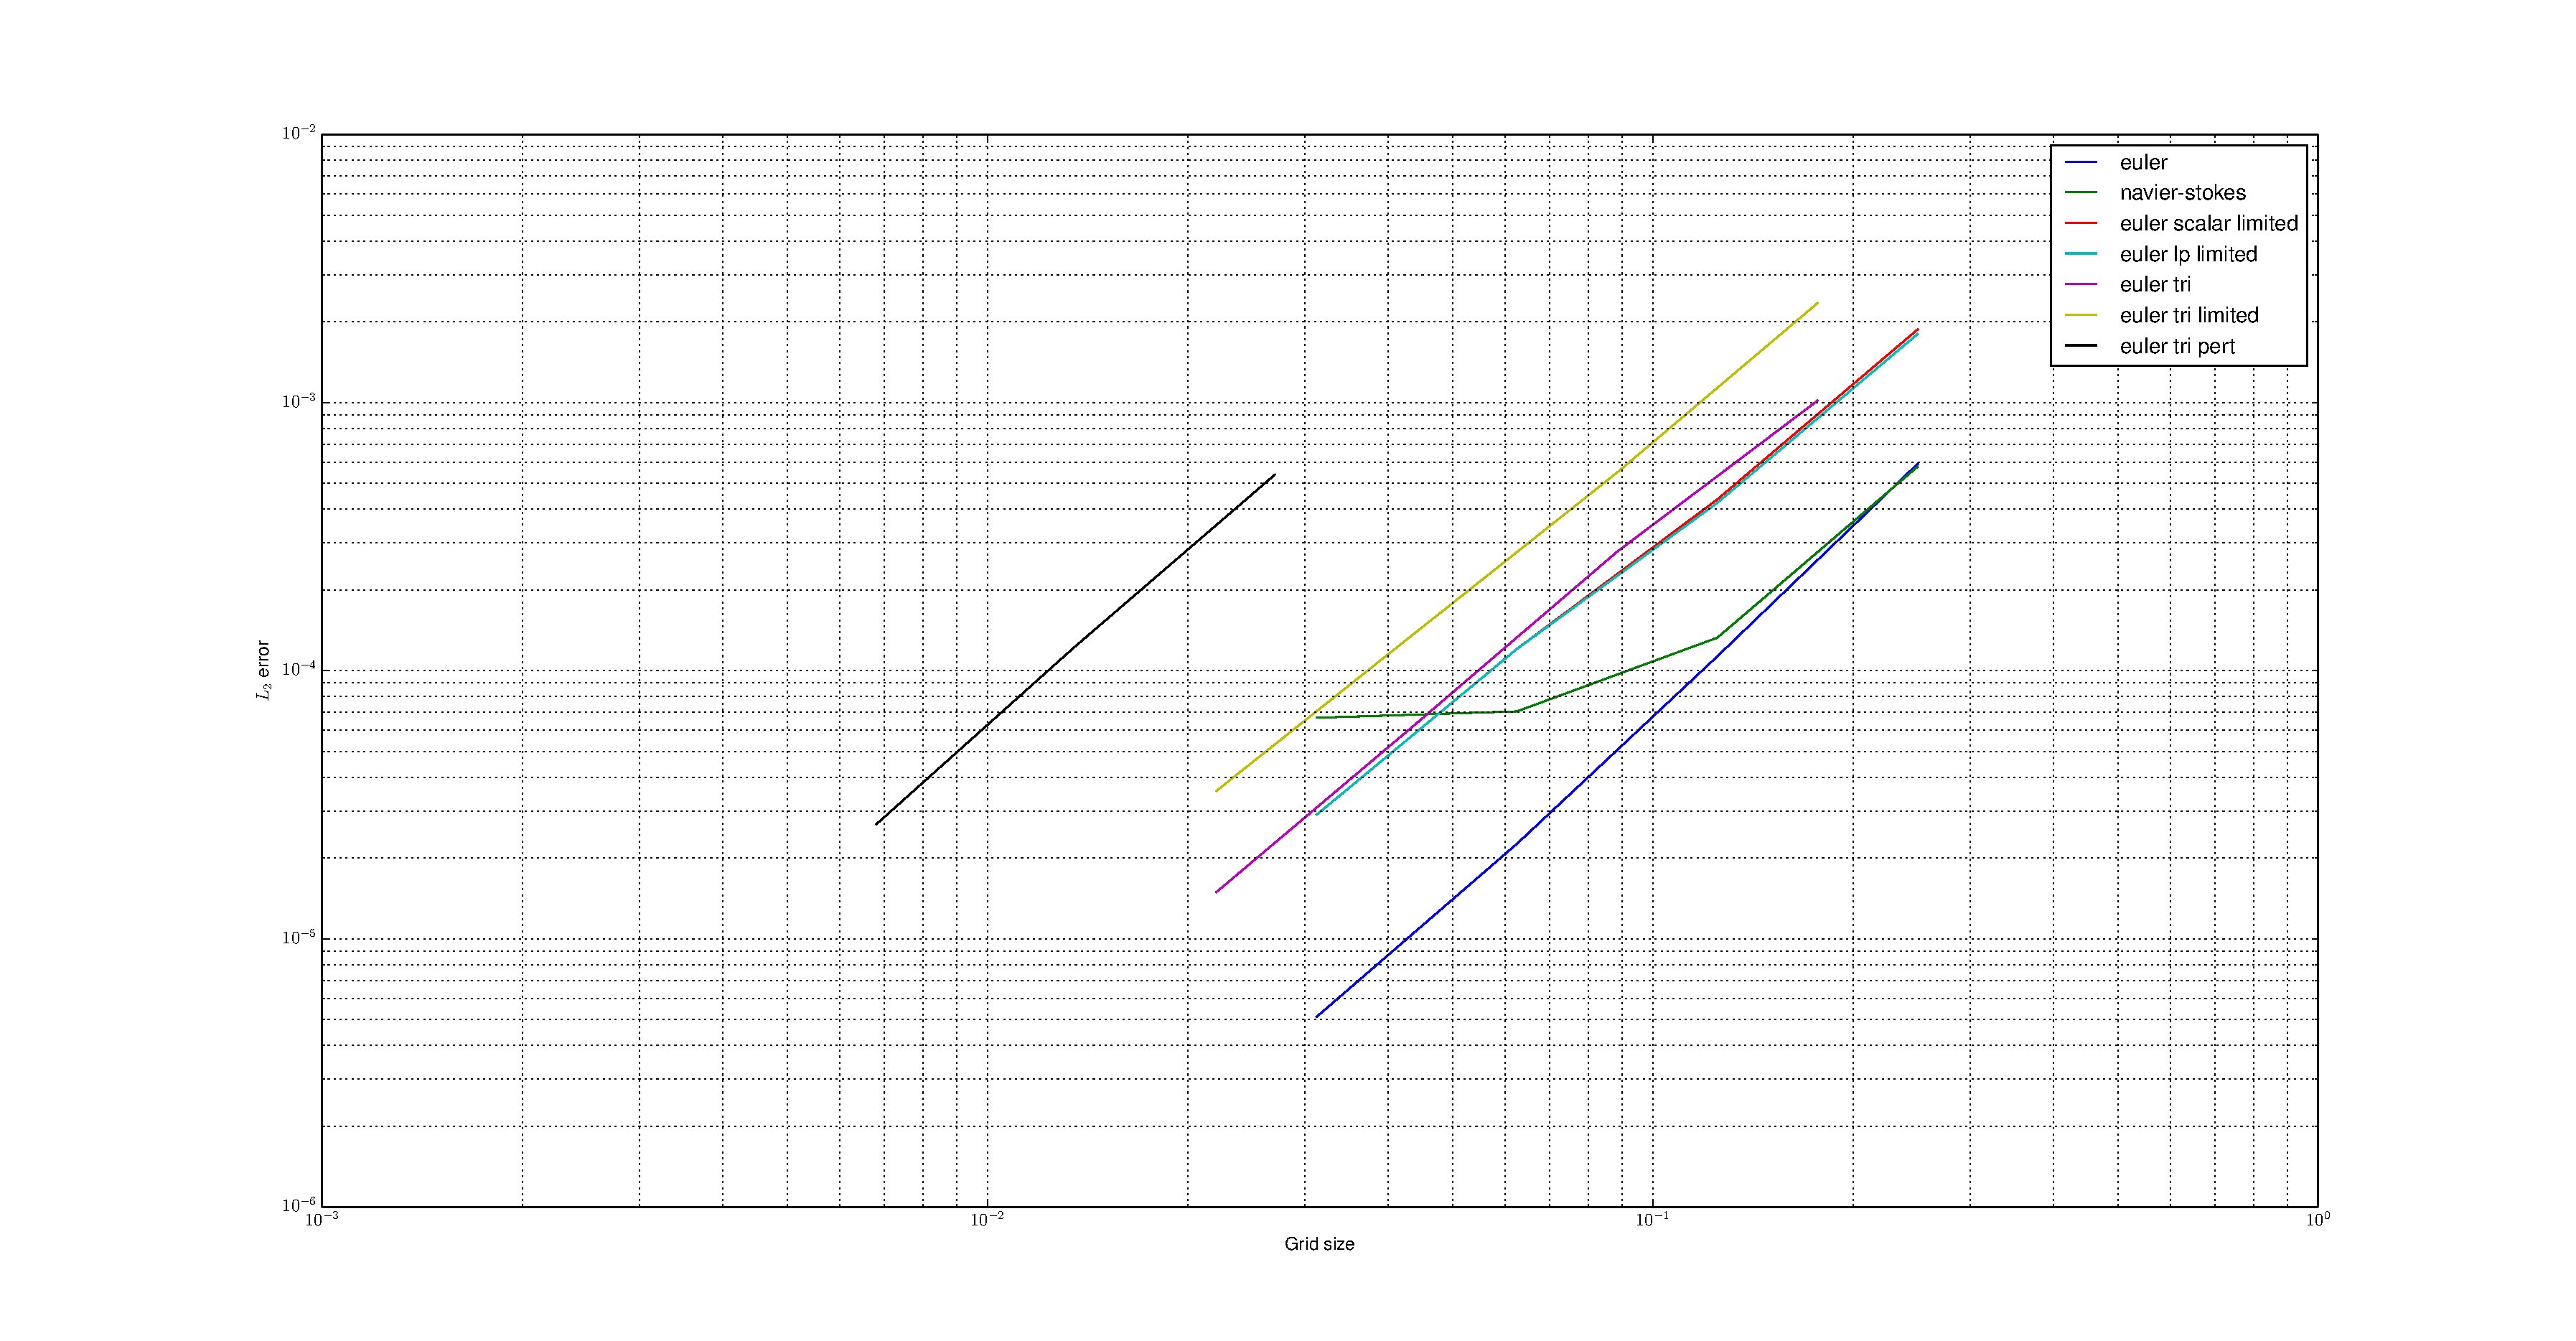
\includegraphics[width=\textwidth]{ConvergencePlot.pdf}
		\end{figure}

		\begin{centering}
		\begin{tabular}[H]{ l | l }
			Test case				 & $L_2$ norm convergence \\ \hline
			$\rho$ euler                & 2.1434294539853114 \\
			$\rho$ euler tri            & 2.093189333389638 \\
			$\rho$ euler tri perturbed  & 2.2192894148572293 \\
			$\rho$ euler tri limited    & 1.9735741877530029 \\
			$\rho$ euler lp tri limited & 2.0581615298644054 \\
			$\rho$ euler limited        & 2.0553411497426697 \\
			$\rho$ euler lp limited     & 2.051432719728797 \\
			$\rho$ ns                   & 2.118701700561286 \\
			$\rho$ ns end               & 0.0794710679455764 \\
			$C_d$ ns flat plat        & 0.5740461311366147 \\
			$C_d$ ns flat plat end    & 2.3796673876043295 \\
		\end{tabular}
		\end{centering}

		The Navier-Stokes convergence was computed using a flat plate test case on a uniform quadrilateral grid. The Manufactured solutions
		were demonstrating very poor convergence while this case showed better than second order by the end. This points to my source term 
		equations being incorrect for the viscous case and will need to be fixed.

\end{document}
